\documentclass[a4paper]{article}
\usepackage[utf8x]{inputenc}
\usepackage[T1,T2A]{fontenc}
\usepackage[russian]{babel}
\usepackage{hyperref}
\usepackage{indentfirst}
\usepackage{color}
\usepackage{listings}
\usepackage{here}
\usepackage{array}
\usepackage{multirow}
\usepackage{graphicx}
\usepackage{caption}

\lstset{ %
extendedchars=\true,
keepspaces=true,
language=C++,					% choose the language of the code
basicstyle=\footnotesize,		% the size of the fonts that are used for the code
numbers=left,					% where to put the line-numbers
numberstyle=\footnotesize,		% the size of the fonts that are used for the line-numbers
stepnumber=1,					% the step between two line-numbers. If it is 1 each line will be numbered
numbersep=5pt,					% how far the line-numbers are from the code
backgroundcolor=\color{white},	% choose the background color. You must add \usepackage{color}
showspaces=false				% show spaces adding particular underscores
showstringspaces=false,			% underline spaces within strings
showtabs=false,					% show tabs within strings adding particular underscores
frame=single,           		% adds a frame around the code
tabsize=4,						% sets default tabsize to 2 spaces
captionpos=b,					% sets the caption-position to bottom
breaklines=true,				% sets automatic line breaking
breakatwhitespace=false,		% sets if automatic breaks should only happen at whitespace
escapeinside={\%*}{*)},			% if you want to add a comment within your code
postbreak=\raisebox{0ex}[0ex][0ex]{\ensuremath{\color{red}\hookrightarrow\space}}
}
\begin{document}	% начало документа

\begin{titlepage}	% начало титульной страницы

	\begin{center}		% выравнивание по центру

		\large Санкт-Петербургский Политехнический Университет Петра Великого\\
		\large Институт компьютерных наук и технологий \\
		\large Кафедра компьютерных систем и программных технологий\\[6cm]
		% название института, затем отступ 6см
		
		\huge Программирование\\[0.5cm] % название работы, затем отступ 0,5см
		\large Отчет по курсовой работе\\[0.1cm]
		\large "Игра Реверси (Отелло)"\\[5cm]

	\end{center}


	\begin{flushright} % выравнивание по правому краю
		\begin{minipage}{0.25\textwidth} % врезка в половину ширины текста
			\begin{flushleft} % выровнять её содержимое по левому краю

				\large\textbf{Работу выполнил:}\\
				\large Бойцов К.С.\\
				\large {Группа:} 13501/4\\
				
				\large \textbf{Преподаватель:}\\
				\large Вылегжанина К.Д.
				

			\end{flushleft}
		\end{minipage}
	\end{flushright}
	
	\vfill % заполнить всё доступное ниже пространство

	\begin{center}
	\large Санкт-Петербург\\
	\large \the\year % вывести дату
	\end{center} % закончить выравнивание по центру

\thispagestyle{empty} % не нумеровать страницу
\end{titlepage} % конец титульной страницы

\vfill % заполнить всё доступное ниже пространство
% Содержание
\tableofcontents
\newpage

\section{Игра Реверси}
\subsection{Задание}
Реализовать настольную игру Реверси.

\subsection{Правила игры}
В игре используется квадратная доска размером 8х8 (все клетки могут быть одного цвета) и 64 специальные фишки, окрашенные с разных сторон в контрастные цвета, например, в белый и чёрный. Клетки доски нумеруются от верхнего левого угла: вертикали - латинскими буквами, горизонтали - цифрами. Один из игроков играет белыми, другой - чёрными. Делая ход, игрок ставит фишку на клетку доски "своим" цветом вверх.

В начале игры в центр доски выставляются 4 фишки: чёрные на d5 и e4, белые на d4 и e5. Первый ход делают чёрные. Далее игроки ходят по очереди.
Делая ход, игрок должен поставить свою фишку на одну из клеток доски таким образом, чтобы между этой поставленной фишкой и одной из имеющихся уже на доске фишек его цвета находился непрерывный ряд фишек соперника, горизонтальный, вертикальный или диагональный (другими словами, чтобы непрерывный ряд фишек соперника оказался "закрыт" фишками игрока с двух сторон). Все фишки соперника, входящие в "закрытый" на этом ходу ряд, переворачиваются на другую сторону (меняют цвет) и переходят к ходившему игроку.

Если в результате одного хода "закрывается" одновременно более одного ряда фишек противника, то переворачиваются все фишки, оказавшиеся на всех "закрытых" рядах.

Игрок вправе выбирать любой из возможных для него ходов. Если игрок имеет возможные ходы, он не может отказаться от хода. Если игрок не имеет допустимых ходов, то ход передаётся сопернику.

Игра прекращается, когда на доску выставлены все фишки или когда ни один из игроков не может сделать хода. По окончании игры проводится подсчёт фишек каждого цвета, и игрок, чьих фишек на доске выставлено больше, объявляется победителем. В случае равенства количества фишек засчитывается ничья.

\subsection{Концепция}
Готовый проект должен предполагать возможность игры двух игроков. 

\subsection{Минимально работоспособный продукт}
Минимальным работоспособным продуктом должно быть консольное приложение, позволяющее играть двоим игрокам.


\subsection{Диаграмма прецедентов использования}

\begin{figure}[H]
	\begin{center}
		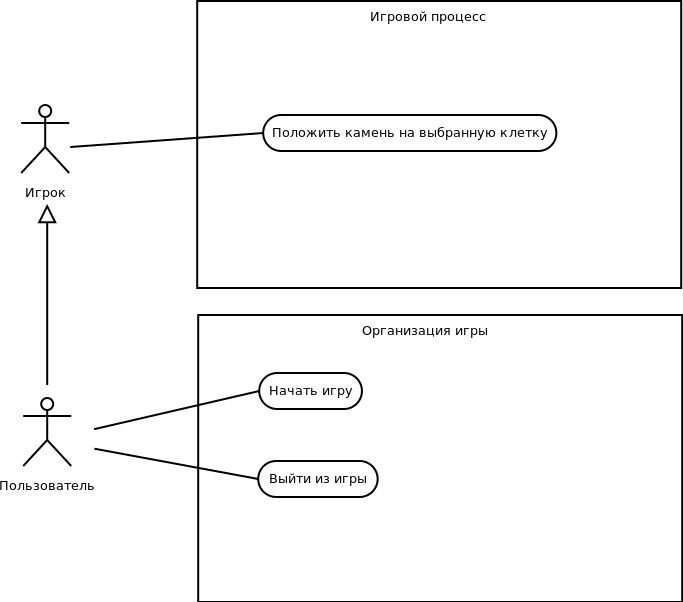
\includegraphics[scale=0.4, height=7cm]{Diagrams/Diagram1}
		\caption{Диаграмма прецедентов использования} 
		\label{pic:Diagram1} % название для ссылок внутри кода
	\end{center}
\end{figure}

\section{Проектрование приложения, реализующего игру Реверси}
Программа разделена на 3 подпроекта: app - консольное приложение, core - библиотека, реализующая модель Жизнь, gui - графическое приложение.

\begin{figure}[H]
	\begin{center}
		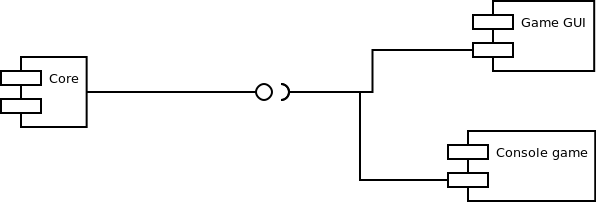
\includegraphics[scale=0.4, height=3cm]{Diagrams/Diagram2}
		\caption{Диаграмма прецедентов использования} 
		\label{pic:Diagram2} % название для ссылок внутри кода
	\end{center}
\end{figure}


\section{Реализация игры Реверси}
\subsection{Версии программ}
Операционная система: Ubuntu 15.10, среда разработки: Qt Creator 3.5.0, компилятор: GCC 4.9.1.


\subsection{Библиотека}
\noindent Основные классы, выделенные в библиотеке:
\begin{itemize}
\item Класс Dot. Реализует клетку. Содержит координаты клетки и её состояние. Присутствуют методы, возвращающие и задающие координаты и состояние клетки.
\item Класс Field. Класс представляет поле модели. Содержит размер поля и двумерный массив клеток.
\item Класс Game. Класc представляет методы, содержащие правила игры.
\end{itemize}

\subsection{Графическое приложение}
Графическое приложение позволяет работать с моделью через окна графического приложения.

\noindent Классы, выделенные в графическом приложении. 
\begin{itemize}
\item Класс MainWindow. Главное окно приложения. Присутствуют кнопки «Новая игра» и «Выход».

\item Класс GrafField. Строит графическую модель поля.
\end{itemize}

\begin{figure}[H]
	\begin{center}
		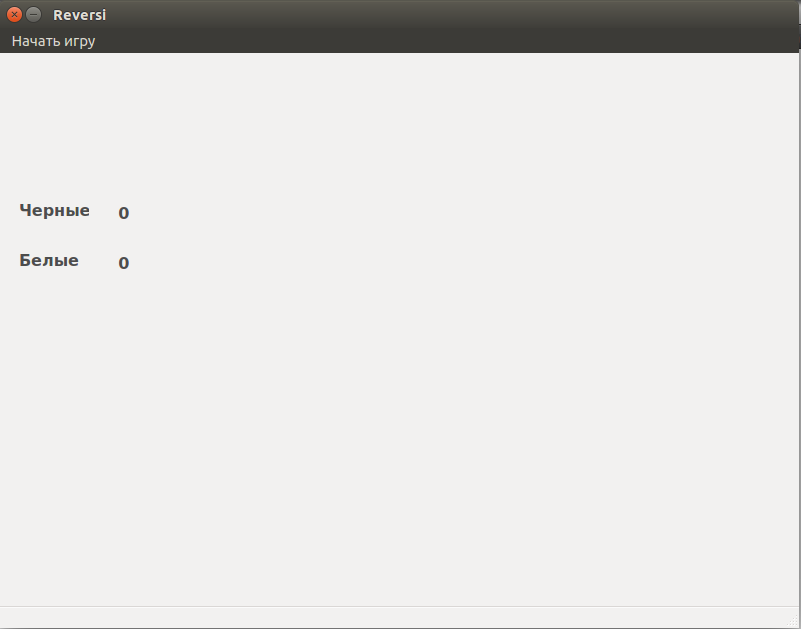
\includegraphics[scale=0.5]{gui}
		\caption{Главное меню графического приложения} 
		\label{pic:graphicsMeinMenu} % название для ссылок внутри кода
	\end{center}
\end{figure}

На рис \ref{pic:graphicsMeinMenu} представлено главное окно приложения. В нём пользователю можно начать новую игру. 

\begin{figure}[H]
	\begin{center}
		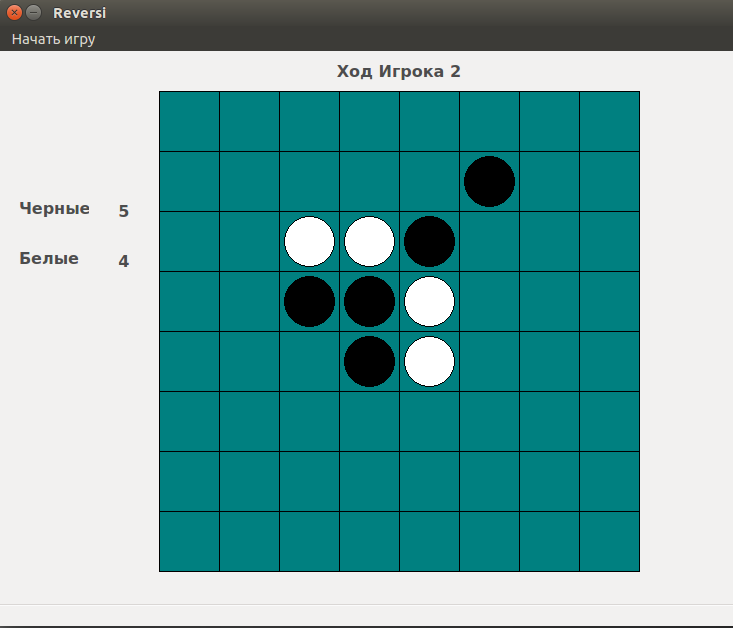
\includegraphics[scale=0.5]{gui2}
		\caption{Игровое поле}
		\label{pic:graphicsField}
	\end{center}
\end{figure}

На рис \ref{pic:graphicsField} представлено игровое поле.

\section{Вывод}
По окончании семестра автор проекта научился делать графический интерфейс с помощью Qt, а также получил опыт работы с большими проектами, содержащими много классов и имеющих как консольное приложение, так и графическое.

\section{Приложение 1. Листинги кода}
\subsection{Консольное приложение}
\lstinputlisting[]
{../source/TheReversiGame/App/main.cpp}
\newpage

\lstinputlisting[]
{../source/TheReversiGame/App/Game.h}
\lstinputlisting[]
{../source/TheReversiGame/App/Game.cpp}
\newpage

\subsection{Графическое приложение}
\lstinputlisting[]
{../source/TheReversiGame/GUI/main.cpp}
\newpage

\lstinputlisting[]
{../source/TheReversiGame/GUI/graffield.h}
\lstinputlisting[]
{../source/TheReversiGame/GUI/graffield.cpp}
\newpage

\lstinputlisting[]
{../source/TheReversiGame/GUI/mainwindow.h}
\lstinputlisting[]
{../source/TheReversiGame/GUI/mainwindow.cpp}
\newpage


\subsection{Библиотека}

\lstinputlisting[]
{../source/TheReversiGame/Core/Game.h}
\lstinputlisting[]
{../source/TheReversiGame/Core/Game.cpp}
\newpage

\lstinputlisting[]
{../source/TheReversiGame/Core/Dot.h}
\lstinputlisting[]
{../source/TheReversiGame/Core/Dot.cpp}
\newpage

\lstinputlisting[]
{../source/TheReversiGame/Core/Board.h}
\lstinputlisting[]
{../source/TheReversiGame/Core/Board.cpp}
\newpage

\end{document}